\section{Process discovery through Grammar Inference} \label{grammar}
Perhaps, the research most relevant to my own was done by Cook \& Wolf in \cite{citeulike:328044}. The authors developed a \textit{``process discovery''} techniques intended to discover process models from event streams. The authors did not really intend to generate a complete model, but rather to generate sub-models that express the most frequent patterns in the event stream. They designed a framework which collects process data from ongoing software process or from history logs, and generates a set of recurring patterns of behavior characterizing observed process. In this work they extended two methods of \textit{grammar inference} from previous work: purely statistical (neural network based \textit{RNet}) and purely algorithmic (\textit{KTail}) as well as developing their own Markovian method (\textit{Markov}). 

\textit{Process discovery}, in the author's opinion, resembles the process of \textit{grammar inference}, which can be defined as the process of inferring a language grammar from the given set (sample) of sentences in this language. In the demonstrated approach, words of the language are atomic events of the dynamic process, whether sentences built from such words, are describing the behavior of a process. Consequently, the inferred grammar of that language is the formal model of the process. Cook \& Wolf expressed such grammars as Finite State Machines (FSMs) and implemented a software tool for the mining of the software process. This tool was successfully tested in an industrial case study.

\begin{figure}[tbp]
   \centering
   \includegraphics[height=70mm]{inference.eps}
   \caption{Process discovery through the grammar inference: panel a) a sample event stream (simple process involving three types of events: Edit, Review, and Checkin); and FNA results obtained by applying three methods of process discovery from Cook \& Wolf \cite{citeulike:328044}.}
   \label{fig:inference}
\end{figure}

The first method extended by the authors, the neural-network based grammar inference, RNet algorithm, defines a recurrent neural network architecture which is trained by the sequences of events. After training, this neural net is able to characterize a current system state by looking on past behavior. Authors extract the FSM from the trained neural network by presenting different strings to it and extracting the hidden neurons activity through observations. Due to the nature of Neural Net, closely related activation patterns are clustered into the same state; therefore, by noting the current pattern, the input token, and the next activation pattern, transitions are recorded and compiled into the inferred FSM.

The second method investigated, is a purely algorithmic KTail method, which was taken from the work of Biermann \& Feldman \cite{citeulike:5120603}. The idea is that a current state is defined by what future behaviors can occur from it. The \textit{future} is defined as the set of next $k$ tokens. By looking at a window of successor events, the KTail algorithm can build the equivalence classes that compose the process model. The authors extensively modified the original KTail algorithm improving the folding in the mined model making to make it more robust to noise.

The Markov based method developed by authors is based on both algorithmic and statistical approaches. It takes to account past and future system behavior in order to guess the current system state. Assuming that a finite number of states can define the process, and that the probability of the next state is based only on the current state (Markov property), the authors built a $n^{th}$-order Markov model using the first and second order probabilities. Once built, the transition probability table corresponding to the Markov model is converted into FSM which is in turn reduced based on the user-specified cut-off threshold for probabilities.

The authors implemented all three of these algorithms in a software tool called \textsc{DaGama} as a plugin for larger software system called Balboa \cite{citeulike:5120757}. By performing benchmarking, Cook \& Wolf found that the Markov algorithm was superior to the two others. RNet was found to be the worst of the three algorithms. 

Overall, while having some issues with the complexity of produced output and noise handling, the authors proved applicability of implemented algorithms to real-world process data by demonstrating an abstraction of the actual process executions and capturing important properties of the process behavior. The major backdraw of the approach, as stated by authors, lies in the inability of the FSMs to model concurrency of processes which limits its applicability to the software development process. Later, Cook et al. in \cite{citeulike:5128143} addressed this limitation.
